% Options for packages loaded elsewhere
\PassOptionsToPackage{unicode}{hyperref}
\PassOptionsToPackage{hyphens}{url}
%
\documentclass[
]{article}
\usepackage{amsmath,amssymb}
\usepackage{iftex}
\ifPDFTeX
  \usepackage[T1]{fontenc}
  \usepackage[utf8]{inputenc}
  \usepackage{textcomp} % provide euro and other symbols
\else % if luatex or xetex
  \usepackage{unicode-math} % this also loads fontspec
  \defaultfontfeatures{Scale=MatchLowercase}
  \defaultfontfeatures[\rmfamily]{Ligatures=TeX,Scale=1}
\fi
\usepackage{lmodern}
\ifPDFTeX\else
  % xetex/luatex font selection
\fi
% Use upquote if available, for straight quotes in verbatim environments
\IfFileExists{upquote.sty}{\usepackage{upquote}}{}
\IfFileExists{microtype.sty}{% use microtype if available
  \usepackage[]{microtype}
  \UseMicrotypeSet[protrusion]{basicmath} % disable protrusion for tt fonts
}{}
\makeatletter
\@ifundefined{KOMAClassName}{% if non-KOMA class
  \IfFileExists{parskip.sty}{%
    \usepackage{parskip}
  }{% else
    \setlength{\parindent}{0pt}
    \setlength{\parskip}{6pt plus 2pt minus 1pt}}
}{% if KOMA class
  \KOMAoptions{parskip=half}}
\makeatother
\usepackage{xcolor}
\usepackage[margin=1in]{geometry}
\usepackage{longtable,booktabs,array}
\usepackage{calc} % for calculating minipage widths
% Correct order of tables after \paragraph or \subparagraph
\usepackage{etoolbox}
\makeatletter
\patchcmd\longtable{\par}{\if@noskipsec\mbox{}\fi\par}{}{}
\makeatother
% Allow footnotes in longtable head/foot
\IfFileExists{footnotehyper.sty}{\usepackage{footnotehyper}}{\usepackage{footnote}}
\makesavenoteenv{longtable}
\usepackage{graphicx}
\makeatletter
\def\maxwidth{\ifdim\Gin@nat@width>\linewidth\linewidth\else\Gin@nat@width\fi}
\def\maxheight{\ifdim\Gin@nat@height>\textheight\textheight\else\Gin@nat@height\fi}
\makeatother
% Scale images if necessary, so that they will not overflow the page
% margins by default, and it is still possible to overwrite the defaults
% using explicit options in \includegraphics[width, height, ...]{}
\setkeys{Gin}{width=\maxwidth,height=\maxheight,keepaspectratio}
% Set default figure placement to htbp
\makeatletter
\def\fps@figure{htbp}
\makeatother
\setlength{\emergencystretch}{3em} % prevent overfull lines
\providecommand{\tightlist}{%
  \setlength{\itemsep}{0pt}\setlength{\parskip}{0pt}}
\setcounter{secnumdepth}{5}
\ifLuaTeX
  \usepackage{selnolig}  % disable illegal ligatures
\fi
\usepackage{bookmark}
\IfFileExists{xurl.sty}{\usepackage{xurl}}{} % add URL line breaks if available
\urlstyle{same}
\hypersetup{
  pdftitle={Reveiwer1\_RhoQ},
  pdfauthor={Sophie Wulfing},
  hidelinks,
  pdfcreator={LaTeX via pandoc}}

\title{Reveiwer1\_RhoQ}
\author{Sophie Wulfing}
\date{2024-06-23}

\begin{document}
\maketitle

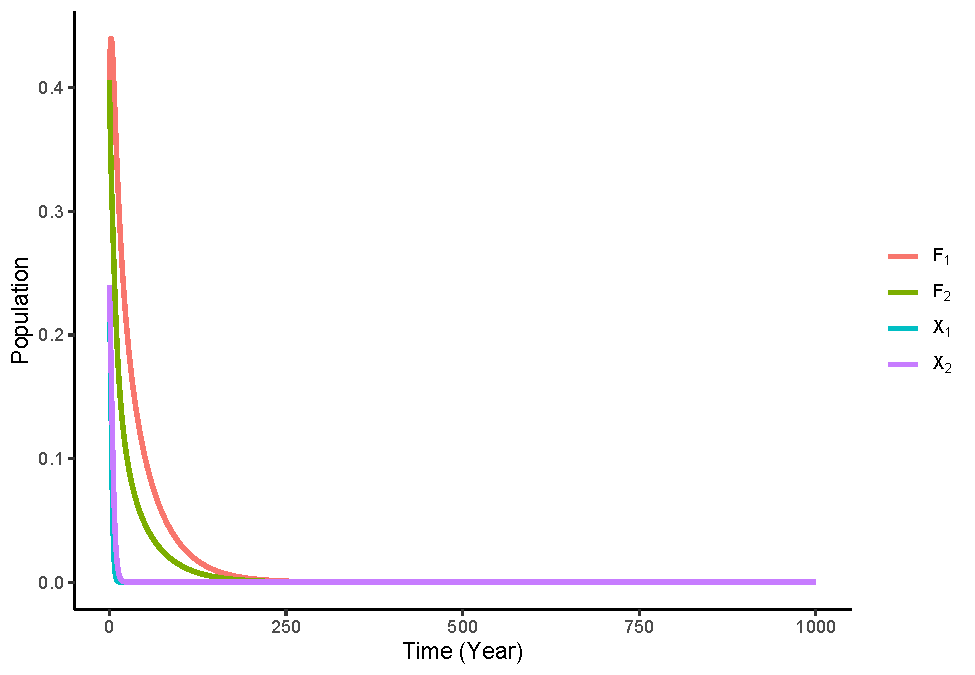
\includegraphics{ReviewerRhoTest_files/figure-latex/Bauch.Coupled-1.pdf}



\begin{figure}
\centering
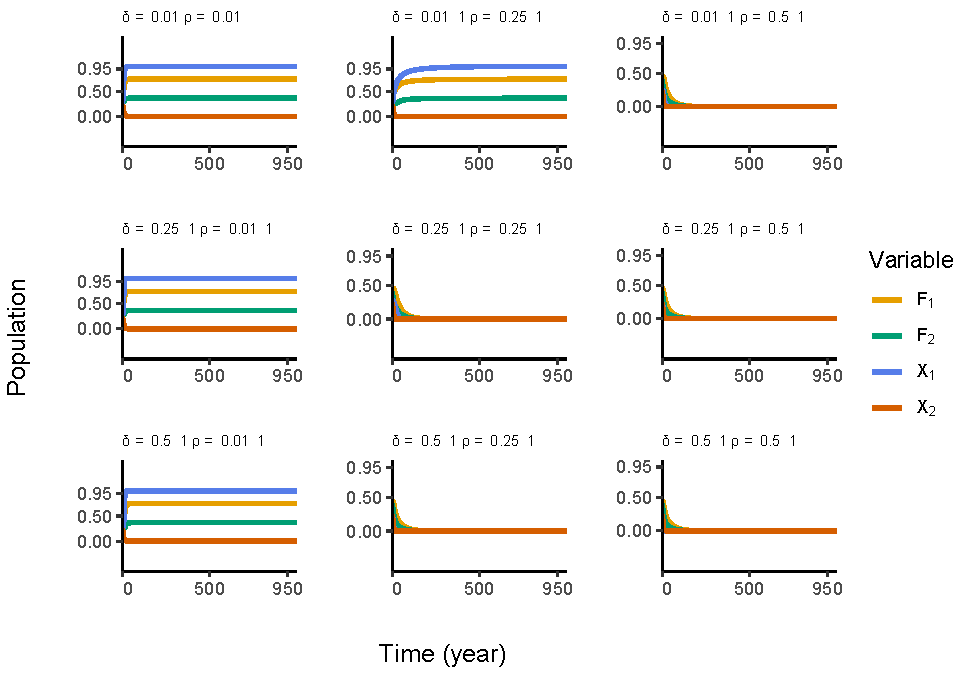
\includegraphics{ReviewerRhoTest_files/figure-latex/influencerho1-1.pdf}
\caption{\label{fig:influencerho1}\(d_1\) and \(\rho_1\) \label{influenceRho1}}
\end{figure}



\begin{figure}
\centering
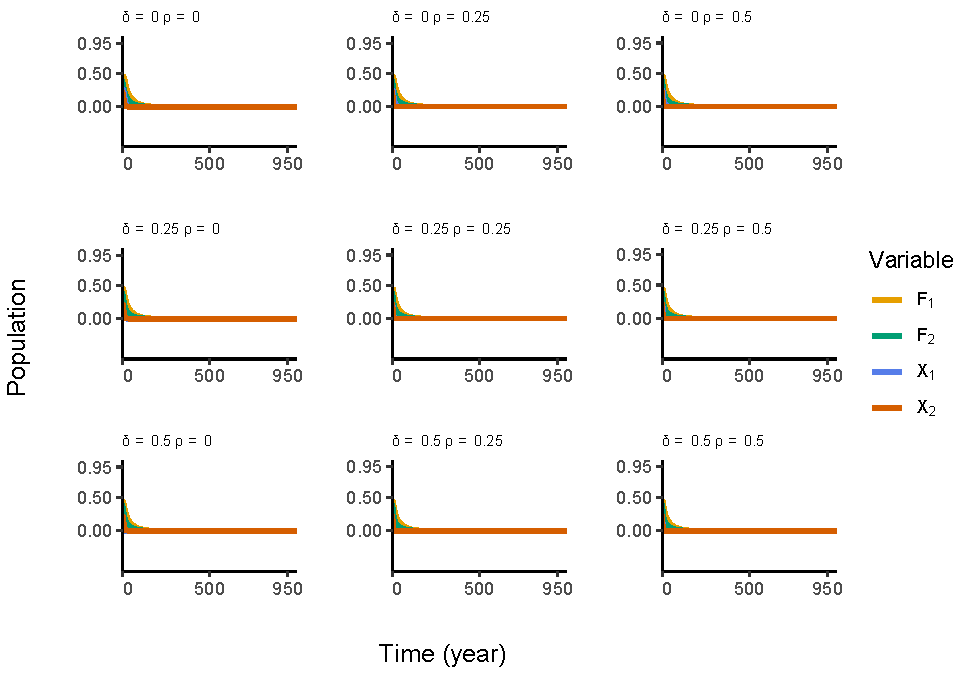
\includegraphics{ReviewerRhoTest_files/figure-latex/influencerho2-1.pdf}
\caption{\label{fig:influencerho2}\(d_1\) and \(\rho_2\) \label{influenceRho2}}
\end{figure}



\begin{figure}
\centering
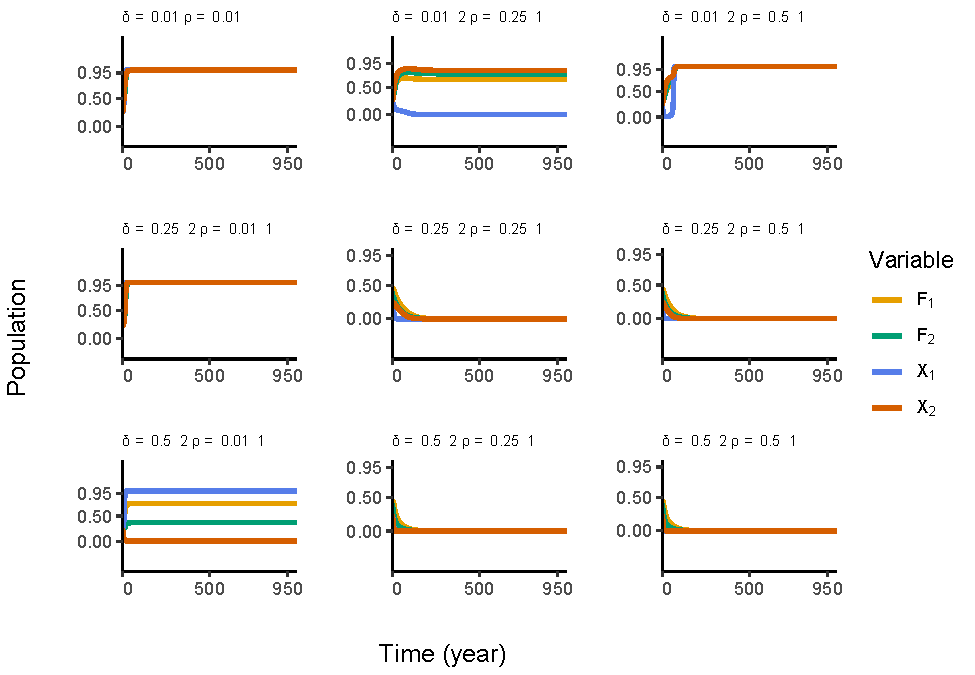
\includegraphics{ReviewerRhoTest_files/figure-latex/influencerho3-1.pdf}
\caption{\label{fig:influencerho3}\(d_2\) and \(\rho_1\) \label{influenceRho3}}
\end{figure}



\begin{figure}
\centering
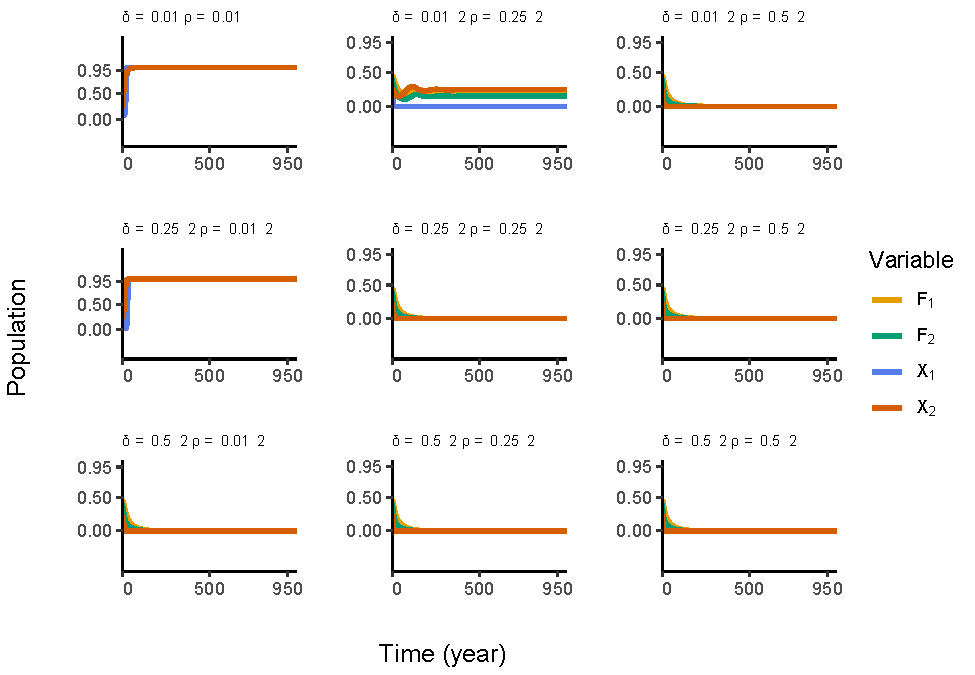
\includegraphics{ReviewerRhoTest_files/figure-latex/influencerho4-1.pdf}
\caption{\label{fig:influencerho4}\(d_2\) and \(\rho_2\) \label{influenceRho4}}
\end{figure}

\newpage



\begin{figure}
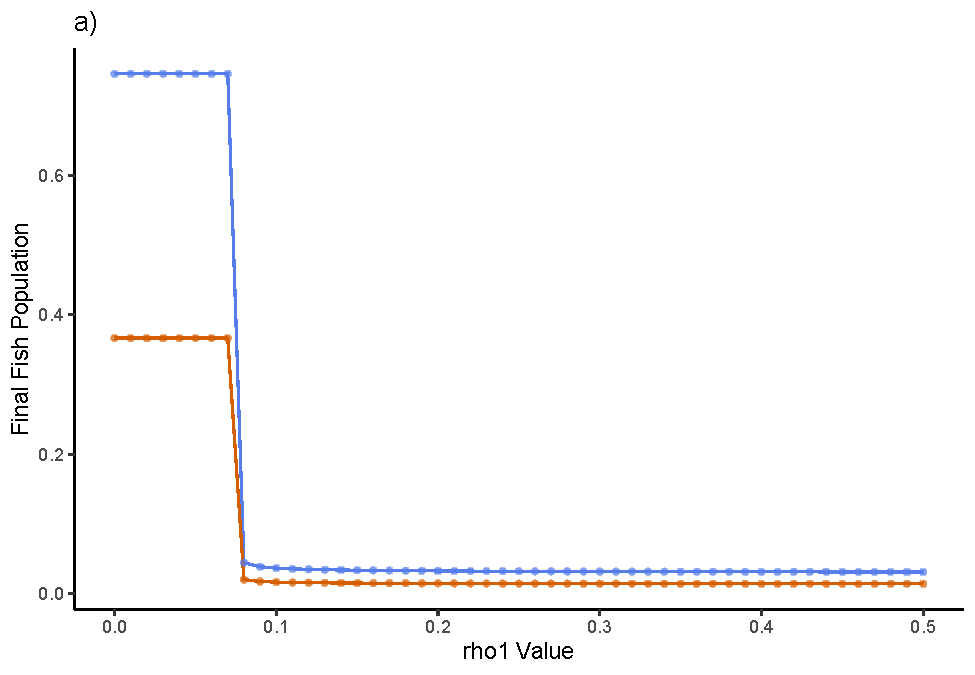
\includegraphics[width=0.5\linewidth]{ReviewerRhoTest_files/figure-latex/rhoExploreGraphEach-1} 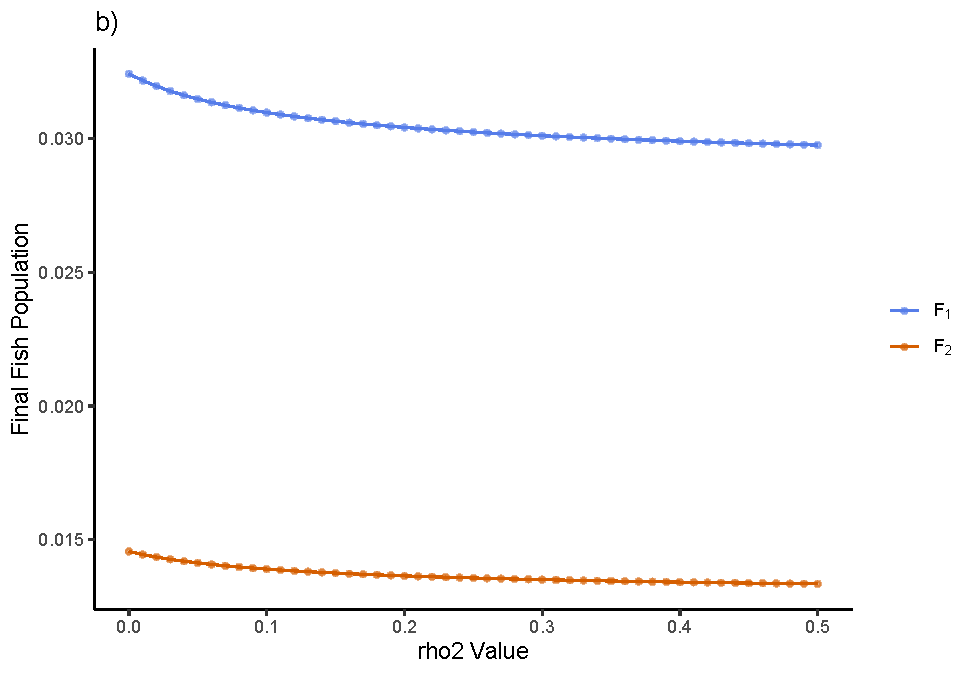
\includegraphics[width=0.5\linewidth]{ReviewerRhoTest_files/figure-latex/rhoExploreGraphEach-2} \caption{Each rho individually. Ok so here's my confusion, above in \ref{influenceAsym} I say that incorporating new information will increase stability but here, as pop 2 (which is unsustainable) listens to pop 1 more, the whole thing crashes. Earlier we said this was because pop 1 is continuing to fish, so therefore encouraging pop 2 to fish more (looking at graph a) \label{rhoExploreGraphEach}}\label{fig:rhoExploreGraphEach}
\end{figure}



\begin{figure}
\centering
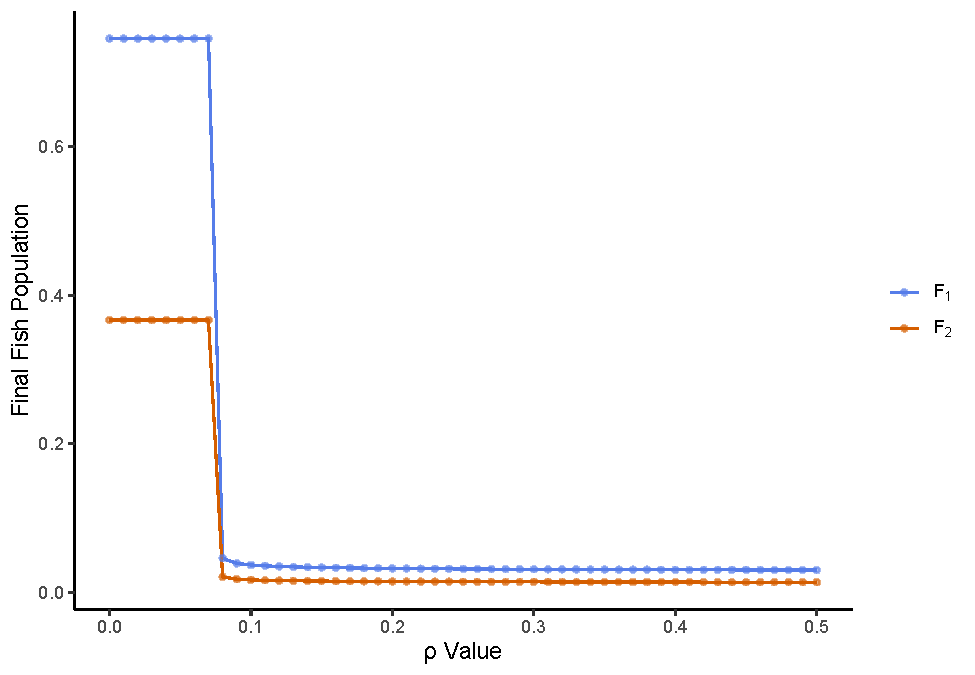
\includegraphics{ReviewerRhoTest_files/figure-latex/rhoExploreGraph-1.pdf}
\caption{\label{fig:rhoExploreGraph}Final fish populations after 100 years in the two-patch fishing model where the \(F_1\) population in patch 1 is fished sustainably but human population 1 has a lower social influence than humans in patch 2, where \(F_2\) is being fished unsustainably. Both \(\rho_1\) and \(\rho_2\) were increased simultaneously. \label{rhoExploreGraph}}
\end{figure}

\end{document}
